\documentclass[a4paper,11pt]{article}
\usepackage[utf8]{inputenc}
\usepackage[italian]{babel}
\usepackage[maxbibnames=99,backend=bibtex]{biblatex}
\usepackage{hyperref}
\usepackage{listings}
\usepackage{color}
\usepackage{graphicx}

\addbibresource{ref.bib}
\graphicspath{ {images/} }

% define the title
\author{Luigi Leonardi}
%\pagestyle{headings}

\title{Relazione Finale Tirocinio}
\date{}


\definecolor{mygreen}{rgb}{0,0.6,0}

\lstset{  
	numbers=left,
	numbersep=5pt,
	commentstyle=\color{mygreen},
	keywordstyle=\color{blue}\ttfamily,
	stringstyle=\color{red}\ttfamily  
}


%link cliccabili
\hypersetup{colorlinks=true, linktoc=all,  linkcolor=black,citecolor=black}

\begin{document}
	% generates the title
	\maketitle
	% insert the table of contents
	\tableofcontents
	
%	\cite{epfl1}
	

\newpage
	\section{Introduzione}
	\subsection{Posit}

	Il Posit è un formato di numero in virgola mobile ideato da John Gustafson\cite{john}, in alternativa allo standard IEEE 754. L'idea di base è fondamentalmente la stessa, anche nei Posit è presente un bit per il segno, dei bit per l'esponente e dei bit per la mantissa, le principali differenze consistono nella presenza di un "super esponente" o regime e nel non avere un numero di bit fissato per quest'ultimo e per la mantissa. \\
	\begin{figure}[h]
	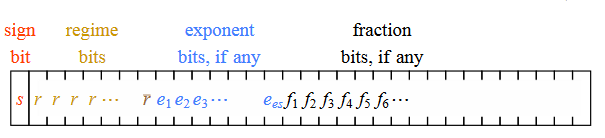
\includegraphics[scale=0.8]{posit}
	\centering
	\caption{"Formato Posit"}
	\end{figure}Il vantaggio nell'avere un super esponente, la cui lunghezza non è definita, permette di ottenere un range di numeri molto più flessibile, il suo contributo è pari a $2^{2^{es}}$ con es il numero di bit dell'esponente\footnote{L'esponente è l'unico campo ad avere una dimensione fissa}, permettendo ad esempio una riduzione del numero di bit assegnati a quest'ultimo campo.\newline Questi bit di regime non sono altro che una sequenza di cifre binarie identiche, terminate dal complemento di esse. \newline Ad esempio: 0001 rappresenta -3, dove 3 è il numero degli 0 ed 1 è il terminatore.\footnote{Regimi che iniziano per 0 sono negativi, per 1 invece sono positivi. Lo 0 è rappresentato come 10} \\
	Non sono inoltre previsti overflow e underflow o la rappresentazione di NaN.
	
	\subsection{Note sui Test}
	Tutti i test svolti sui Posit sono stati effettuati sfruttando la libreria in C++ BFP\cite{libbfp} 
	implementando, dove necessario, le funzionalità mancanti.\newline I Posit scelti sono stati a 32/64 bit, con 0 bit di esponente\footnote{Ha senso non utilizzare bit di esponente, in quanto si sfrutta il super esponente}, dove non specificato diversamente.
	
%	\subsection{Cippi}
%	\ldots{} ora e' in distilleria.
\newpage
\section {Test su Moltiplicazione}
\subsection{Accuratezza}

Questo test vuole dimostrare che a parità di bit utilizzati, 32 in questo caso, i Posit risultano essere più precisi nel rappresentare i risultati di prodotti, rispetto ad un Float a 32 bit.\\
In questo particolare caso sono stati impiegati Posit [32,3], ossia 32 bit totali, di cui 3 di esponente.
\subsubsection{Svolgimento}
Il test consiste nel creare 9 array, 6 per gli operandi e 3 per i risultati, di una dimensione compresa nell'ordine dei milioni: \begin{itemize}
	\item 3 di Posit [32,3]
	\item 3 di Float a 32 bit 
	\item 3 di Double a 64 bit come riferimento
\end{itemize} Il passo successivo consiste nel popolare gli array degli operandi, operazione che viene svolta partendo dai Double sfruttando una funzione che genera dei numeri in modo pseudo-casuale, per poi provvedere a riempire gli altri semplicemente operando le necessarie conversioni.\\
Successivamente sono stati eseguiti i vari prodotti i cui risultati sono stati collocati nel terzo array di ciascun tipo. Infine, per poter confrontare il tutto, i risultati sono stati riportarti in Double e ne è stata fatta la differenza, in modulo, rispetto al riferimento.\\\\ Definisco: \begin{center}  $\Delta_i$(Posit) = $|PositRes_i - DoubleRes_i|$  \\ $\Delta_i$(Float)  = $|FloatRes_i - DoubleRes_i|$ \end{center} 
Dove FloatRes e PositRes sono il risultato del prodotto, fra Float e Posit rispettivamente, convertiti in double. \\Se $\Delta_i$(Posit) $<$ $\Delta_i$(Float) i Posit sono più precisi dei Float per questo indice.\\ Se $\Delta_i$(Posit) $>$ $\Delta_i$(Float) i Float sono più precisi dei Posit per questo indice.

\subsubsection{Conclusioni}
Dai risultati dei test svolti, i Posit si sono rivelati essere più precisi dei Float nel $\approx56$\% dei casi. Sono risultati pari merito nel $\approx16$\% dei casi.\\
I risultati risultano essere in linea con le aspettative, in quanto una maggiore precisione, a parità di dimensione, è imputabile ad un numero maggiore di bit disponibili per la mantissa, rispetto ai Float. 

\subsubsection{Codice}
\begin{lstlisting}[language=C++]
//Funzione per Numeri Random
double genererateNumber(){
	double tmp = (double)rand()/(double)RAND_MAX;
	
	return (tmp*2000);
}

\end{lstlisting}
\newpage
\subsection{Tempi}
Lo scopo di questo test è incentrato sul capire se, oltre ad esservi dei vantaggi a livello di precisione, vi sono dei vantaggi a livello di prestazioni nell'eseguire moltiplicazioni.\\
I Posit utilizzati sono del tipo [32-3]. 


\subsubsection{Svolgimento}
Per poter effettuare dei test che non avvantaggiassero i Float, sfruttando supporto hardware, è stata sfruttata la libreria SoftFloat\cite{softfloat} la quale implementa i Float interamente via software.\\
Lo svolgimento del test è simile al precedente, vengono creati 6 array di dimensione nell'ordine dei milioni \begin{itemize}
	\item 2 di Float
	\item 2 di SoftFloat a 32 bit
	\item 2 di Posit[32,3]
\end{itemize}
I primi due vengono popolati con numeri generati in modo pseudo-casuale, mentre i rimanenti 4 vengono riempiti convertendo, nei rispettivi formati, i numeri ottenuti precedentemente. Per poter ottenere i tempi è stata sfruttata la funzione clock\_gettime(), la quale restituisce il timestamp di sistema. Salvando il timestamp ad inizio e fine elaborazione, durante il quale vengono eseguite le moltiplicazioni fra i due array, si riescono ad ottenere per differenza i tempi di lavoro per ciascun tipo di numero.

\subsubsection{Conclusioni}
Come potevamo aspettarci i Float con supporto hardware, sono stati $\approx11$ volte più veloci dei SoftFloat, mentre il divario è addirittura maggiore con i Posit. Per quanto riguarda questi ultimi, sono stati più lenti di $\approx2$ volte rispetto ai SoftFloat.\\ Anche questo risultato era prevedibile, in quanto i Posit non sono altro che una generalizzazione dei Float, avendo aggiunto dei campi a lunghezza variabile.

\begin{table}[ht]
	\centering
	\begin{tabular}{l*{3}{c}r}
		Test              &Float Hardware & SoftFloat & Posit  \\
		\hline
		Moltiplicazione		& 1 & $\approx11$ & $\approx22$   		\\
		\hline
	\end{tabular}
	\caption{Moltiplicazione fra 2 numeri}
\end{table}


\newpage
\subsubsection{Codice}
\begin{lstlisting}[language=C++]
//Funzione per calcolo tempi Posit
double doTestPosit(unsigned int *X,unsigned int *Y,unsigned long n)
{

	auto p1 = Posit(32, 3);
	auto p2 = Posit(32, 3);    
	
	timespec start, stop;
	
	clock_gettime( CLOCK_REALTIME, &start);
	
	for(unsigned long i=0;i<n;i++){
		p1.setBits(X[i]);
		p2.setBits(Y[i]);
	
		p1.mul(p2);
	}
	
	clock_gettime( CLOCK_REALTIME, &stop);
	
	double res = BILLION*( stop.tv_sec - start.tv_sec ) + 
	( stop.tv_nsec - start.tv_nsec );
	
	return res;

}


\end{lstlisting}
\newpage
\section{Test su Sigmoide}
\subsection{Introduzione}
Una caratteristica dei Posit con 0 bit di esponente, come osservato da Isaac Yonemoto, è che risulta molto facile e conveniente, a livello computazionale, calcolare la funzione sigmoidea, infatti bastano dei semplici shift e not. Essa trova largo impiego nell'ambito delle reti neurali e machine learning.
\\Per poter eseguire i seguenti test, è stato necessario implementare una funzione di conversione da Posit[32-0] a Float, in quanto la libreria ne risulta essere sprovvista.

\subsection{Accuratezza}
Il primo test che è stato eseguito è di tipo numerico, ossia data la funzione  $ f(x) = \frac {1}{1 + e^{-x}} $, sono stati confrontati i risultati con quelli restituiti dalla sigmoide ottenuta mediante manipolazione dei bit.

\subsubsection{Svolgimento}

Per questo tipo di test vengono generati un numero di Float, nell'ordine delle migliaia, in modo pseudo-casuale nel range -30 e 30, e ne viene calcolata la sigmoide sfruttando prima la funzione con l'esponenziale, e successivamente, dopo aver convertito il numero in Posit, l'altra.
Infine è stato eseguito un plot di tutti i risultati su MatLab ed ottenuto il seguente grafico:

\begin{figure}[h]
	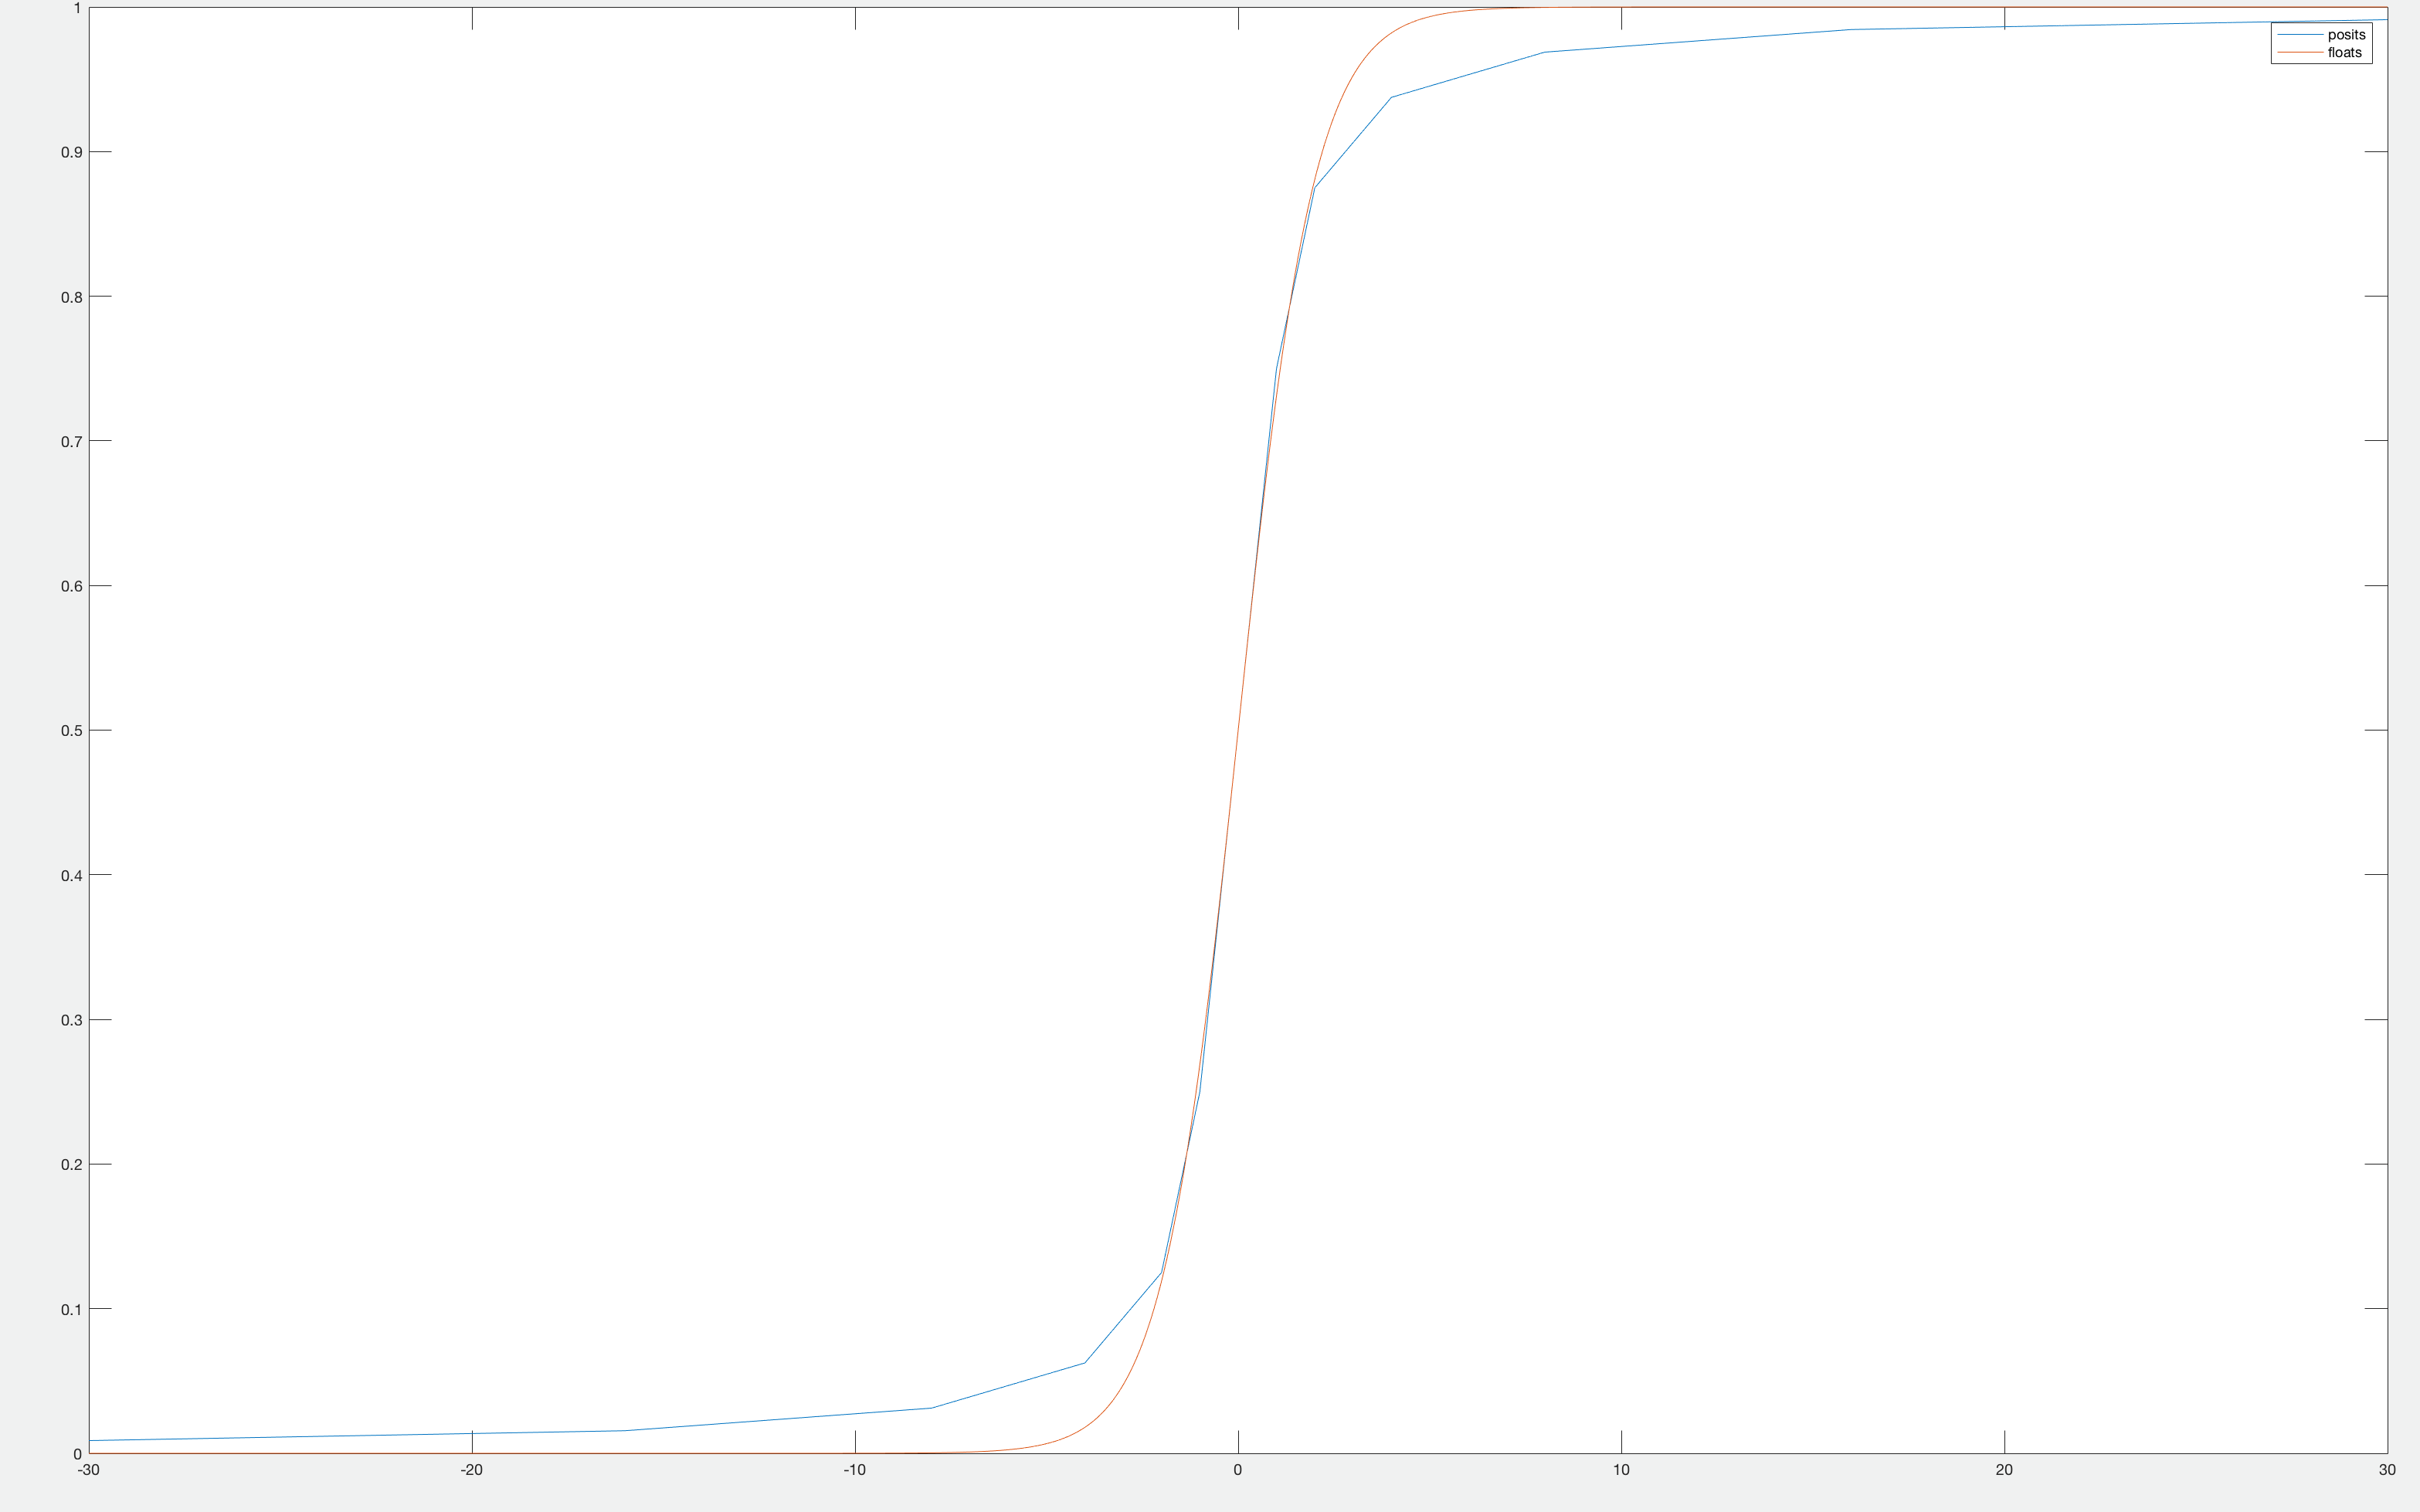
\includegraphics[scale=0.15]{sigmoide_2}
	\centering
	\caption{"Sigmoide"}
\end{figure}

\subsubsection{Conclusioni}
Come si può evincere dalla figura, il grafico ottenuto con i  Posit sembra essere una spezzata che segue l'andamento della sigmoide con i Float, inoltre i due grafici si vanno a sovrapporre nell'origine. In generale comunque possiamo affermare che effettivamente questo tipo di manipolazione sui bit, ha fornito una approssimazione della sigmoide.

\subsubsection{Codice}

\begin{lstlisting}[language=C++]
//Sigmoide con Float
float sigmoid(float &x){
	return 1/(exp(-x)+1);
}

//Sigmoide con Posit
unsigned int sigmoid(unsigned int bits){
	bits = bits ^ 0x80000000;
	bits = bits >> 2;
	return bits;
}


//Conversione da Posit[32-0] a Float
float Posit::subconv(){
	union {
		float f;
		uint32_t bits;
	};
	bits=0;
	
	if((mBits & 0xFFFFFFFF) == 0)
	return 0.0f;
	signed char c = (signed char)(regime());
	c+= 127;
	unsigned int esponente = (unsigned int)(c);	
	
	esponente = esponente<<23;
	bits = bits | esponente;
	unpacked_t aup = unpack_posit(mBits, mNbits, mEs);
	unsigned int fr_ = aup.frac;
	
	fr_ = fr_>>9;
	bits = bits | fr_;
	int segno = aup.neg;
	if(segno == 0)
		bits &= 0x7FFFFFFF;
	else
		bits |= 0x80000000;
	
	return f;
}
\end{lstlisting}
\newpage
\subsection{Tempi}

Una volta dimostrato che possiamo approssimare la sigmoide, il passo successivo è quello di provare che effettivamente vi sia un risparmio tangibile nell'eseguire i calcoli. \\
Questo test, suddiviso in più parti, effettua diversi confronti, sui tempi di elaborazione, fra sigmoide su Posit e sigmoide ottenuta in vari modi sui Float.

\subsubsection{Parte 1}

Il primo confronto eseguito è stato con la funzione sigmoide esponenziale  $ f(x) = \frac {1}{1 + e^{-x}} $, la stessa utilizzata nel test numerico.\\
Esso consiste nel generare un milione di Float pseudo-casuali, e di scriverli su file sia come Float che come Posit sotto forma di bit, il tutto per evitare di falsare il test a sfavore di questi ultimi, in quanto nel tempo di elaborazione vi sarebbe anche il tempo di conversione. \\
Una volta acquisiti i dati da file, per ciascun tipo, viene impiegata la funzione clock\_gettime(), la quale viene richiamata prima e dopo aver finito di calcolare la sigmoide su tutti i dati.\\
Successivamente è stato ripetuto lo stesso esperimento, incrementando gradualmente il numero di elementi, per verificare se l'eventuale margine fosse influenzato dalle dimensioni, nello specifico lo step scelto è stato di 10 mila, con numero massimo di 5 milioni.

\begin{figure}[h]
	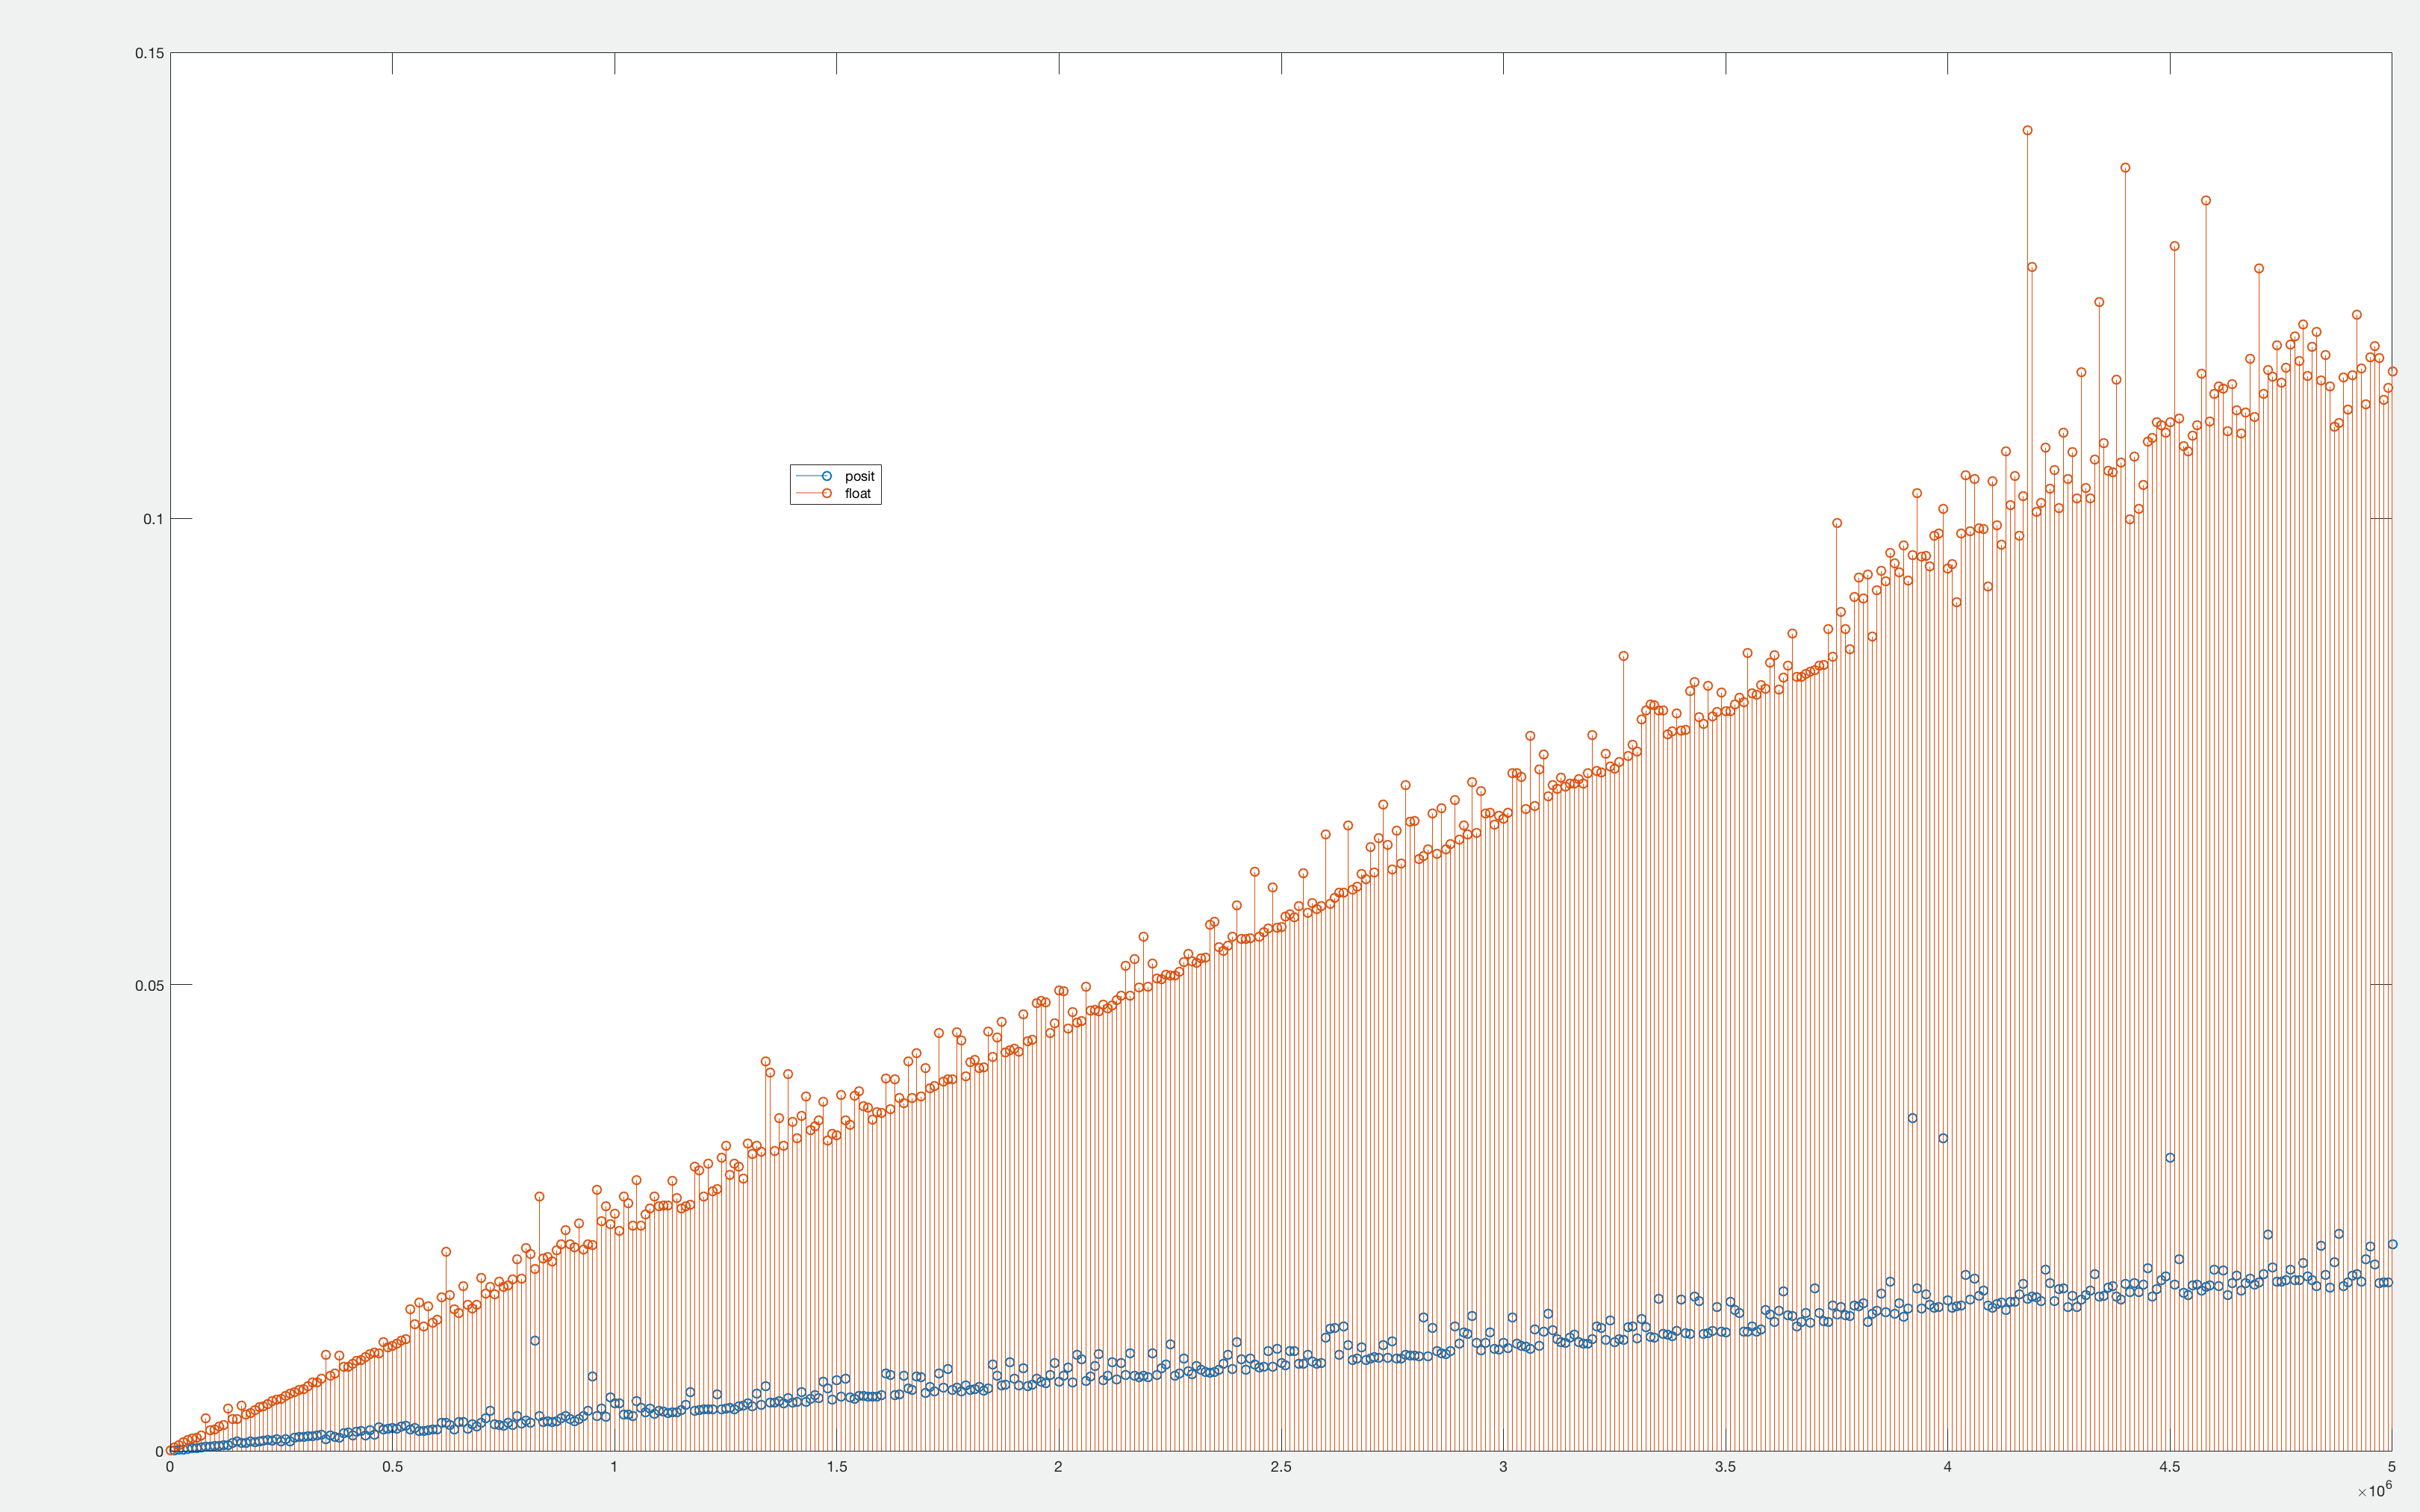
\includegraphics[scale=0.15]{tempi}
	\centering
	\caption{"Tempi all'aumentare degli elementi"}
\end{figure}


\subsubsection{Parte 1 - Esito}


I risultati hanno evidenziato che la funzione, calcolata mediante manipolazione di bit, quindi impiegando solamente la ALU del processore, è più rapida di $\approx1.5-1.8$\ volte su un campione di 1 milione di elementi. \\
Per quanto riguarda l'incremento, come si può evincere dalla Figura 3, il tempo di elaborazione aumenta linearmente all'aumentare del numero degli elementi in entrambi i casi, di conseguenza possiamo affermare che il vantaggio rimane pressoché costante.

 
\subsubsection{Parte 2}

In questa seconda parte è stato scelto come metro di paragone, invece della curva logistica su Float, una sua versione approssimata ottenuta mediante quanto descritto nell'articolo "A Fast, Compact Approximation of the Exponential Function"\cite{afast}. In particolare questo algoritmo ci permette di ottenere una approssimazione di $e^{x}$, sfruttando il fatto che i Float, utilizzano una rappresentazione del tipo $2^x$. Il vantaggio consiste nel fatto che il tutto è ottenuto operando solamente semplici operazioni sui bit.\\
La metodologia del test è medesima a prima.
\subsubsection{Parte 2 - Esito}

I risultati mostrano che per calcolare la sigmoide con i Posit ci si impiega in media $\approx4.9-5.1$ volte in meno. Di conseguenza nonostante l'aver adoperato questo tipo di approssimazione, risulta essere essere sconveniente l'utilizzo dei Float.

\subsubsection{Parte 3}
L'ultimo confronto che eseguito, è stato usando come riferimento una versione della sigmoide che non fa uso di espoenziali $f(x) = \frac{x}{\sqrt{1+x^{2}}}$, quindi in teoria ancora più rapida da calcolare.\\
Anche in questo caso la metodologia del test è medesima ai precedenti.


\subsubsection{Parte 3 - Esito}

I risultati hanno visto di nuovo i Posit trionfare, questa volta sono risultati essere $\approx1.4-1.6$ volte più veloci rispetto ai Float.
\newpage


%\newpage
\subsubsection{Codice}
\begin{lstlisting}[language=C++]
//Test per Posit
double doTestPosit(unsigned int *posit_array,unsigned long n)
{
	auto p = Posit(32, 0);
	timespec start, stop;
	clock_gettime( CLOCK_REALTIME, &start);
	for(unsigned long i=0;i<n;i++){
		sigmoid(posit_array[i]);	
	}
	clock_gettime( CLOCK_REALTIME, &stop);
	double res = BILLION*( stop.tv_sec - start.tv_sec ) 
	+ ( stop.tv_nsec - start.tv_nsec ); 
	return res;
}
//Sigmoide su Posit
unsigned int sigmoid(unsigned int bits){
	bits = bits ^ 0x80000000;
	bits = bits >> 2;
	return bits;
}
//Sigmoide Curva Logistica
float sigmoid(float &x){
	return 1/(exp(-x)+1);
}
//Sigmoide Esponenziale Approssimata
float sigmoid(float &x){
	return 1/(EXP_V(-x)+1);
}
//Sigmoide Approssimata con Float
float sigmoid(float &x){
	return x/sqrtf((float)(x*x+1));
}
//Approssimazione Esponenziale
#define EXPA (1048576/LN2) 		
#define EXPC 60801 			
#define EXP_V(y) (eco.n.i = EXPA*(y) + (1072693248 - EXPC), eco.d)

\end{lstlisting}
\newpage
\subsection{Conclusioni}
I Posit sono stati gli assoluti vincitori sui tempi di calcolo della sigmoide, senza perdere troppo in accuratezza, rendendoli particolarmente interessanti in ambienti in cui ne viene fatto un largo impiego. Inoltre vista la presenza del superesponente, si potrebbe anche pensare di utilizzare meno bit per i dati, non rinunciando eccessivamente sulla precisione o sul range di rappresentabilità.

\begin{table}[ht]
	\centering
	\begin{tabular}{l*{3}{c}r}
		Test              & Posit &Float Hardware \\
		\hline
		Curva Logistica 				& 1 & $\approx1.5-1.8$    	\\
		Esp. Approssimato  				& 1 & $\approx4.9-5.1$		\\
		Sigmoide senza Esp.           	& 1 & $\approx1.4-1.6$		\\
		\hline
	\end{tabular}
	\caption{Tempi di calcolo della sigmoide nei tre casi}
\end{table}


\newpage
\section{Divisione e Moltiplicazione mediante regime}
\subsection{Introduzione}

Lavorando con Posit con 0 bit di esponente, il "superesponente" $(2^{2^{es}})^{regime}$ viene notevolmente semplificato, in quanto $2^{2^{0}} = 2 => 2^{regime} $ esattamente come nei Float. L'unica differenza consiste nel fatto che il regime non è un campo a dimensione fissa.\\ L'idea è stata quella di sfruttare questa caratteristica dei Posit 0, per implementare moltiplicazioni e divisione, per potenze del 2, semplicemente intervenendo sul regime. Il grande vantaggio consiste nel fatto che essendo esso composto da una sequenza di bit uguali, incrementarne o decrementarne il valore è relativamente semplice e poco costoso!\\
Ad esempio, dato un Posit-0: 0 001 00000\footnote{Regime = -2; Mantissa = 0}, il quale rappresenta +0.25, se volessimo dividerlo per 2, basterebbe aggiungere uno 0 al regime, ottenendo quindi 0 0001 0000\footnote{Regime = -3; Mantissa = 0} = +0.125

\subsection{Accuratezza}

Dopo aver implementato le funzioni che eseguono rispettivamente moltiplicazione e divisione, è stata testata l'accuratezza confrontando i risultati, utilizzando come riferimento i Double. \\
Nello specifico sono stati confrontati il delta fra il riferimento e i risultati ottenuti eseguendo lo stesso calcolo su Posit e Float.

\subsubsection{Risultati} 

Su un campione di 1 milione di numeri non è stata evidenziata alcuna differenza fra i risultati ottenuti con i Float e con i Posit nel 100\% dei casi.\\
Il risultato è giustificabile con il fatto che, eliminando il "superesponente" il Posit diventa un Float con una mantissa a dimensione variabile.

\subsection{Tempi}
Una volta dimostrato che non vi è alcun vantaggio, in termini di accuratezza, sono stati effettuate verifiche per capire quanto fosse il guadagno in termini computazionali.\\
Il test è stato svolto su un campione di 1 milione di elementi, sfruttando la funzione clock\_gettime(), come già fatto in precedenza.
\subsubsection{Risultati}

Dai dati emersi i Float risultano essere più veloci di $\approx 2-2.5$ volte rispetto ai Posit nelle divisioni, mentre nelle moltiplicazioni il divario aumenta fino a $\approx 3$ volte.\\
Per quanto possa sembrare strano ad un primo impatto, un risultato del genere è del tutto normale, in quanto le divisioni e moltiplicazioni, per potenze del 2, sui Float risultano essere ancora più semplici, in quanto basta semplicemente incrementare (o decrementare) l'esponente, il che è ulteriormente facilitato dalla loro natura "statica".

\begin{table}[ht]
	\centering
	\begin{tabular}{l*{3}{c}r}
		Test              				& Float Hardware &Posit \\
		\hline
		Moltiplicazione 				& 1 & $\approx2.0-2.5$    	\\
		Divisione		  				& 1 & $\approx3.0$		\\
		\hline
	\end{tabular}
	\caption{Moltiplicazione e Divisione per potenze del 2}
\end{table}



\subsubsection{Codice}
\begin{lstlisting}[language=C++]
//Funzione per calcolare i tempi di esecuzione
double doTestPosit(unsigned int *X,unsigned long n)
{
	auto p1 = Posit(32, 0);  
	timespec start, stop;
	
	clock_gettime( CLOCK_REALTIME, &start);
	for(unsigned long i=0;i<n;i++){
		p1.setBits(X[i]);	
		p1.mul_p2(4);			//moltiplico per 16
	}
	
	clock_gettime( CLOCK_REALTIME, &stop);
	
	double res = BILLION*( stop.tv_sec - start.tv_sec ) + 
	( stop.tv_nsec - start.tv_nsec );
	
	return res;
}
//Conversione da Posit a Double
double Posit::subconv64(){
	union {
	double d;
	uint64_t bits;
	};
	
	bits=0;
	if( (mBits & 0xFFFFFFFF) == 0)
		return 0.0f;

	int regime_bits = regime();
	int16_t espo16 = (uint16_t)regime_bits;
	espo16 = espo16 &(0x07FF);
	espo16+=1023;
	espo16 = espo16 &(0x07FF);			//elimino eventuale overflow
	uint64_t espo64 = espo16;
	espo64 = espo64 << (64-12);
	
	if(regime_bits < 0 ){
		regime_bits *=-1;
		regime_bits++;
	}
	else if(regime_bits > 0){
		regime_bits+=2;
	} else if(regime_bits == 0){
		regime_bits = 2;	
	}
		
	regime_bits++; 			//per il segno
	
	uint64_t mask = -1;
	mask = mask >>regime_bits;
	uint64_t bit_veri = 0;
	Posit p = isNeg() ? neg() : *this;
	for (int i = POSIT_SIZE - 1; i >= POSIT_SIZE - mNbits; i--) {
		bit_veri = bit_veri | ((p.mBits >> i) & 1);
		
		if(i > POSIT_SIZE - p.mNbits)
			bit_veri = bit_veri << 1;
	}
	uint64_t frazione = bit_veri & mask;
	frazione = frazione << regime_bits;
	frazione = frazione >> 12;
	
	bits = bits | espo64;
	bits = bits | frazione;
	
	if(isNeg()){
		bits = bits | 0x8000000000000000;
	}
}

\end{lstlisting}

\newpage
\section{Conclusioni}
Nel complesso i Posit si sono rivelati un'ottima alternativa alle soluzioni attualmente impiegate, soprattutto dal punto di vista della flessibilità, basti pensare all'assenza di under o overflow, e sarebbe davvero interessante vederne una loro implementazione hardware, per poterne testare a pieno le potenzialità senza essere vincolati a delle implementazioni software. Inoltre la sua versione a 0 bit di esponente, ha mostrato caratteristiche davvero particolari, come ad esempio la possibilità di calcolare la sigmoide a costo "nullo", che meriterebbero ulteriori analisi.

\newpage

\section{Appendice}
\subsection{Conversione Posit - Float}
Due funzioni che meritano una menzione particolare sono quelle destinate ad effettuare la conversione da Posit 0 a Float e a Double. Esse non sono tuttora presenti nella libreria bfp\cite{libbfp}, e quindi ho dovuto implementarle per lo svolgimento dei vari test.\\ L'idea di base dietro la loro realizzazione, consiste nel fatto che con 0 bit di esponente, il regime non è nient'altro che l'esponente dei Float/Double, ad eccezione di una conversione da complemento a 2, a rappresentazione con bias. Di conseguenza il tutto si riduce ad estrapolare i vari campi, dinamici nei Posit, e convertirli nella dimensione fissa del formato di destinazione.

\subsection{Moltiplicazione e Divisione mediante regime}

Sebbene l'idea dietro questo metodo possa sembrare semplice e veloce, la sua implementazione richiede diversa logica. Nello specifico il caso che necessita di maggiori attenzioni, è quando il regime cambia di segno, ossia ne ho uno positivo, ad esempio +1, e si vuole dividere il numero per 8, ottenendo quindi come regime -2. Questo, per struttura stessa dei Posit comporta notevoli cambiamenti: variano il numero di bit occupati dal regime, nello specifico aumentano, ed inoltre i bit del regime passano da essere una sequenza di 1 terminati da 0, a 0 seguiti da un 1.\footnote{Per poter inserire 0 o 1 in accordo al segno del regime, viene sfruttato un signed integer, nel quale se viene effettuato uno shift a destra, avviene una ricopiatura del primo bit}
Nell'implementazione realizzata, il tutto è gestito eliminando il vecchio regime, mediante shift a sinistra, per poi creare ed inserire quello nuovo mediante shift a destra. Naturalmente il tutto è valido anche nel caso in cui si passi da un regime negativo ad uno positivo, mediante moltiplicazione.\\
Infine bisogna anche considerare che nel caso in cui il Posit fosse negativo, prima di potervi estrarre regime o comunque svolgervi qualunque tipo di operazione, bisogna eseguirne il complemento e sommarvi uno, aggiungendo un ulteriore overhead.\\
E' inoltre possibile effettuare lo stesso ragionamento sui Float o sui Double, nei quali basta incrementare o decrementare l'esponente per ottenere una moltiplicazione o una divisione. Il tutto è inoltre semplificato dal fatto che non vi sono casi particolari da considerare, come il cambio regime.

\subsection{Approssimazione esponenziale su Posit}
Come illustrato nell'articolo di Nicol N. Scharaudolph, il concetto chiave consiste nel mettere un intero y all'interno del campo esponente di un Float, per eseguire $2^{y}$, avendo l'accortezza di sommargli il bias. Questa operazione è ripetibile sia su Posit 0 che non; nel primo caso andrebbe convertito l'intero in regime\footnote{A livello pratico l'intero massimo che sarà elevabile a potenza sarà molto piccolo, in quanto per rappresentare un numero n, bisogna usare almeno n+1 bit}, mentre nel secondo basta solamente porlo nel campo esponente, non vi è neanche la necessità di sommarvici il bias, dato che questo campo utilizza come rappresentazione il complemento a 2.\\
Quindi il numero y, usando un Double, dovrà essere sommato a 1023 e shiftato a sinistra di 20 cifre, ossia $i = 2^{20}(y+1023)$, dove i rappresenta le 32 cifre più significative del Double.
Il problema sorge quando vogliamo elevare un numero non intero, infatti eseguendo lo shift una parte della mantissa di y finirà dentro la mantissa del Double. Nell'articolo viene spiegato che questa cosa è positiva in quanto approssima correttamente l'elevazione a potenza. \\Nel caso di Posit 0 non può funzionare perché bisognerebbe convertire tutto il Posit nel formato del regime, e data la sua natura, non è possibile. Nel caso di Posit normali il tutto non funziona perché dentro il campo esponente andrebbero a finirci parte di regime e parte dell'esponente, i quali hanno 2 rappresentazioni diverse fra loro.
Inoltre data la natura non statica dei Posit, ogni volta bisognerebbe calcolare il numero di shift da fare in base al regime.

\subsection{Perché SoftFloat?}
Inizialmente la strada intrapresa, per svolgere i confronti fra Posit e Float, senza l'impiego dell'FPU, consisteva nell'utilizzare dei flag specifici del compilatore g++, per escludere l'impiego di quest'ultima. Nonostante numerosi tentativi, il risultato, controllato osservando il codice assembly generato dal compilatore, è stato solamente la disabilitazione di SSE. La scelta è quindi ricaduta su SoftFloat, una libreria scritta in C\footnote{Per far linkare la libreria dei Posit in C++ e SoftFloat in C, viene sfruttata la direttiva extern "C"} la quale implementa completamente in software i Float, permettendo dunque confronti più equi.

\newpage
%	\nocite{articolo1}
	
	\printbibliography[title=Bibliografia]

	

\end{document}